\documentclass[a4paper, titlepage,12pt]{article}
\usepackage[swedish,english]{babel}
\usepackage{listings}
\usepackage{verbatimbox}
\usepackage{xcolor}
\usepackage{pgfplots}
\usepackage{tikz}
\usepackage{amsmath}
\usepackage{float}
\usetikzlibrary{datavisualization}
\definecolor{codegreen}{rgb}{0,0.6,0}
\definecolor{codepurple}{rgb}{0.5,0,0.5}
\definecolor{backcolor}{rgb}{0.97,0.97,0.97}
\lstdefinestyle{mystyle}{
	commentstyle=\color{codegreen},
	keywordstyle=\color{magenta},
	numberstyle=\color{gray}\ttfamily\footnotesize,
	backgroundcolor=\color{backcolor},
	basicstyle=\ttfamily\footnotesize,
	stringstyle=\color{codepurple},
	numbers=left,
	tabsize=4
}
\lstset{style=mystyle}

\title{Computer Vision\\Assignment 1 \& 2}
\author{Adam Temmel (adte1700)}
\date{\today}

\begin{document}
\maketitle

\section*{Assignment 1}
	\subsubsection*{Derive a camera's field of view $\theta$ as a function of focal length $f$ and sensor width $w$.}

	For this assignment, I found that the book had a figure which illustrated the relationship between $theta$, $f$ and $w$.

	\begin{figure}[h!]
		\begin{center}
			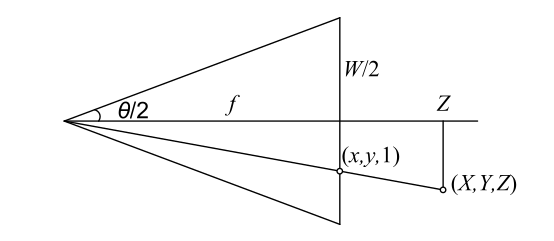
\includegraphics[scale=0.5]{./projection.png}
			\caption{Figure illustrating the relationship between $f$, $\theta$ and $w$.}
			\label{img-fov}
		\end{center}
	\end{figure}

	From what is presented in \textit{figure~\ref{img-fov}}, the following calculations can be performed.

	\begin{center}
		$\frac{w}{2f} = tan(\frac{\theta}{2})$\\
		$\implies tan^{-1}(\frac{w}{2f}) = \frac{\theta}{2}$\\
		$\implies  2 \cdot tan^{-1}(\frac{w}{2f}) = \theta$
	\end{center}

\subsubsection*{Allow two different cameras with sensor with $w_1$ and $w_2$ to have the same focal length $f$. Plot their respective field of view $\theta_1$ and $\theta_2$ in a single graph, to illustrate how field of view varies as a function of focal length for different cameras e.g. a smartphone (smaller sensor) and a DSL (larger sensor)}

The plot in question is presented below.
 
\begin{figure}[H]
\begin{center}
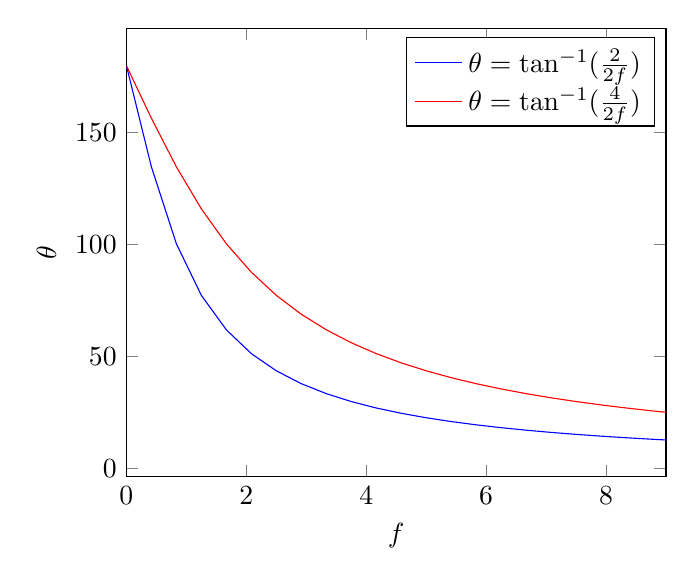
\begin{tikzpicture}
		\begin{axis}[
			xlabel={$f$},
			ylabel={$\theta$},
			domain=0:10,
			xmin=0,
			xmax=9,
		]
			\addplot[color=blue] {2 * atan(2/(2*x))};
			\addplot[color=red] {2 * atan(4/(2*x))};
			\addlegendentry{$\theta = \tan^{-1}(\frac{2}{2f})$};
			\addlegendentry{$\theta = \tan^{-1}(\frac{4}{2f})$};
		\end{axis}
\end{tikzpicture}
\end{center}
	\caption{Plot describing the change in field of view ($\theta$) based upon the change in focal length ($f$) for lenses of width $2$ (blue line) and $4$ (red line)}
\end{figure}

\subsubsection*{Evaluate how the distance between the projected points $|x_2 - x_1|$ varies as a function of focal lengths $f$ and depth $z$.}

	For this exercise, I found that the formula presented in the course slides to perform a perspective projection helped out the most.

	\begin{center}
		$\begin{bmatrix}
			1 & 0 & 0 & 0\\
			0 & 1 & 0 & 0\\
			0 & 0 & 1/f & 0
		\end{bmatrix}
		\begin{bmatrix}
			x \\
			y \\
			z \\
			1
		\end{bmatrix}
		= \begin{bmatrix}
			x \\
			y \\
			z/f
		\end{bmatrix}
		= \begin{pmatrix}
			f \frac{x}{z} & f \frac{y}{z}
		\end{pmatrix}
		$
	\end{center}

	To get a better feel for the effect the formula had on different points with different X-values, I also toyed with the idea of plotting a minor comparison.

	\begin{center}
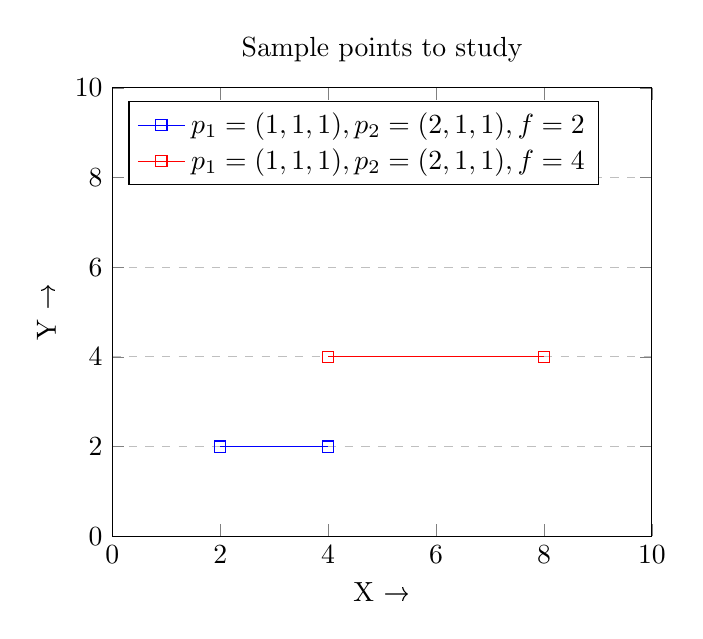
\begin{tikzpicture}
\begin{axis}[
    title={Sample points to study},
    xlabel={X →},
    ylabel={Y →},
    xmin=0, xmax=10,
    ymin=0, ymax=10,
    xtick={0,2,4,6,8,10},
    ytick={0,2,4,6,8,10},
    legend pos=north west,
    ymajorgrids=true,
    grid style=dashed,
]

\addplot[
    color=blue,
    mark=square,
    ]
    coordinates {
		(2,2)
		(4,2)
    };
	\addlegendentry{$p_1 = (1, 1, 1), p_2 = (2, 1, 1), f = 2$}

\addplot[
    color=red,
    mark=square,
    ]
    coordinates {
		(4,4)
		(8,4)
    };
	\addlegendentry{$p_1 = (1, 1, 1), p_2 = (2, 1, 1), f = 4$}
    
\end{axis}
\end{tikzpicture}
	\end{center}
	Conclusion:

	Given $f > 0$, $z_1 = z_2 > 0$ and $y_1 = y_2$, the distance between the projected points $a$ and $b$ would be:
	\begin{center}
	$dx = \frac{f}{z}|x_1-x_2|$
	\end{center}

\subsubsection*{Reflection}

Two things that suprised me a bit regarding the topics covered this week was partially the emphasis on linear algebra throughout the (sometimes rather math heavy) chapters of the book. I have always viewed linear algebra as the mathematical tool for expressing 3D relations between geometric shapes, but, as the book reminded me, most, if not all operations have a 2D counterpart which, depending on the use case, may be more relevant for certain topics within computer vision. The second thing that surprised was the eventual prevalence of computer vision related technologies in systems with rather constrained resources. While researching topics for the first seminar, I stumbled upon a list mentioning some applications of computer vision, which briefly mentioned its presence within NASA's Curiosity rover. I have always viewed computer vision as a rather resource heavy subject, with most algorithms being likely to reach an algorithmic complexity of at least $O(width \cdot height)$, so it was surprising to see that you can find a subset of the topic within a 200MHz CPU positioned somewhere on mars.

\section*{Assignment 2}

\subsubsection*{Solve exercise Ex. 3.10: Separable filters (page 182 in the cource book) in a program language of your choosing.}

The first language I could think of with image decoding/encoding tools as a part of the standard library was Go, which also ended up being the language I implemented the assignment in.\\

The first problem I needed to solve was the implementation of a kernel.

\begin{lstlisting}[language=Go]
type Kernel struct {	// Datatype representing the kernel
	Modifiers []float64
	Width, Height int
}
// Function for extracting an individual weight in the kernel
func (k *Kernel) GetModifier(x, y int) float64 {
	return k.Modifiers[x + y * k.Width]
}
// Function for evaluating a new pixel value
func (k *Kernel) EvalPixel(in *image.NRGBA, x, y int) color.RGBA {
	rSum, gSum, bSum := 0.0, 0.0, 0.0
	halfWidth, halfHeight := k.Width / 2, k.Height / 2
	pt := in.Bounds().Max
	w, h := pt.X, pt.Y
	for i := -halfWidth; i <= halfWidth; i++ {
		for j := -halfHeight; j <= halfHeight; j++ {
			iX, iY := i + x, j + y
			if iX >= 0 && iX < w && iY >= 0 && iY < h {
				clr := in.NRGBAAt(iX, iY)
				r, g, b := clr.R, clr.G, clr.B
				mod := k.GetModifier(i + halfWidth,
					j + halfHeight)
				rSum += (mod * float64(r))
				gSum += (mod * float64(g))
				bSum += (mod * float64(b))
			}
		}
	}
	return color.RGBA{uint8(Round(rSum)),uint8(Round(gSum)),
		uint8(Round(bSum)), 255,
	}
}
\end{lstlisting}

\lstinline{EvalPixel} was then called once for each pixel in the original image, with the value assigned to its corresponding position in a new image. I was originally not pleased with how weak the blur produced from the proposed blur kernel appeared, so I made some slight modifications to it:

\begin{lstlisting}[language=Go]
c2 := 1.0/25.0
k := Kernel{	// 5x5 box blur kernel
	Modifiers: []float64{
		c2, c2, c2, c2, c2,
		c2, c2, c2, c2, c2,
		c2, c2, c2, c2, c2,
		c2, c2, c2, c2, c2,
		c2, c2, c2, c2, c2,
	},
	Width: 5,
	Height: 5,
}
out := k.Apply(img)	// Apply the kernel on the image once
// Reapply the kernel to achieve a stronger blur effect
for i:= 0; i < 20; i++ {
	out = k.Apply(out)
}
\end{lstlisting}

\begin{figure}[h!]
	\begin{center}
	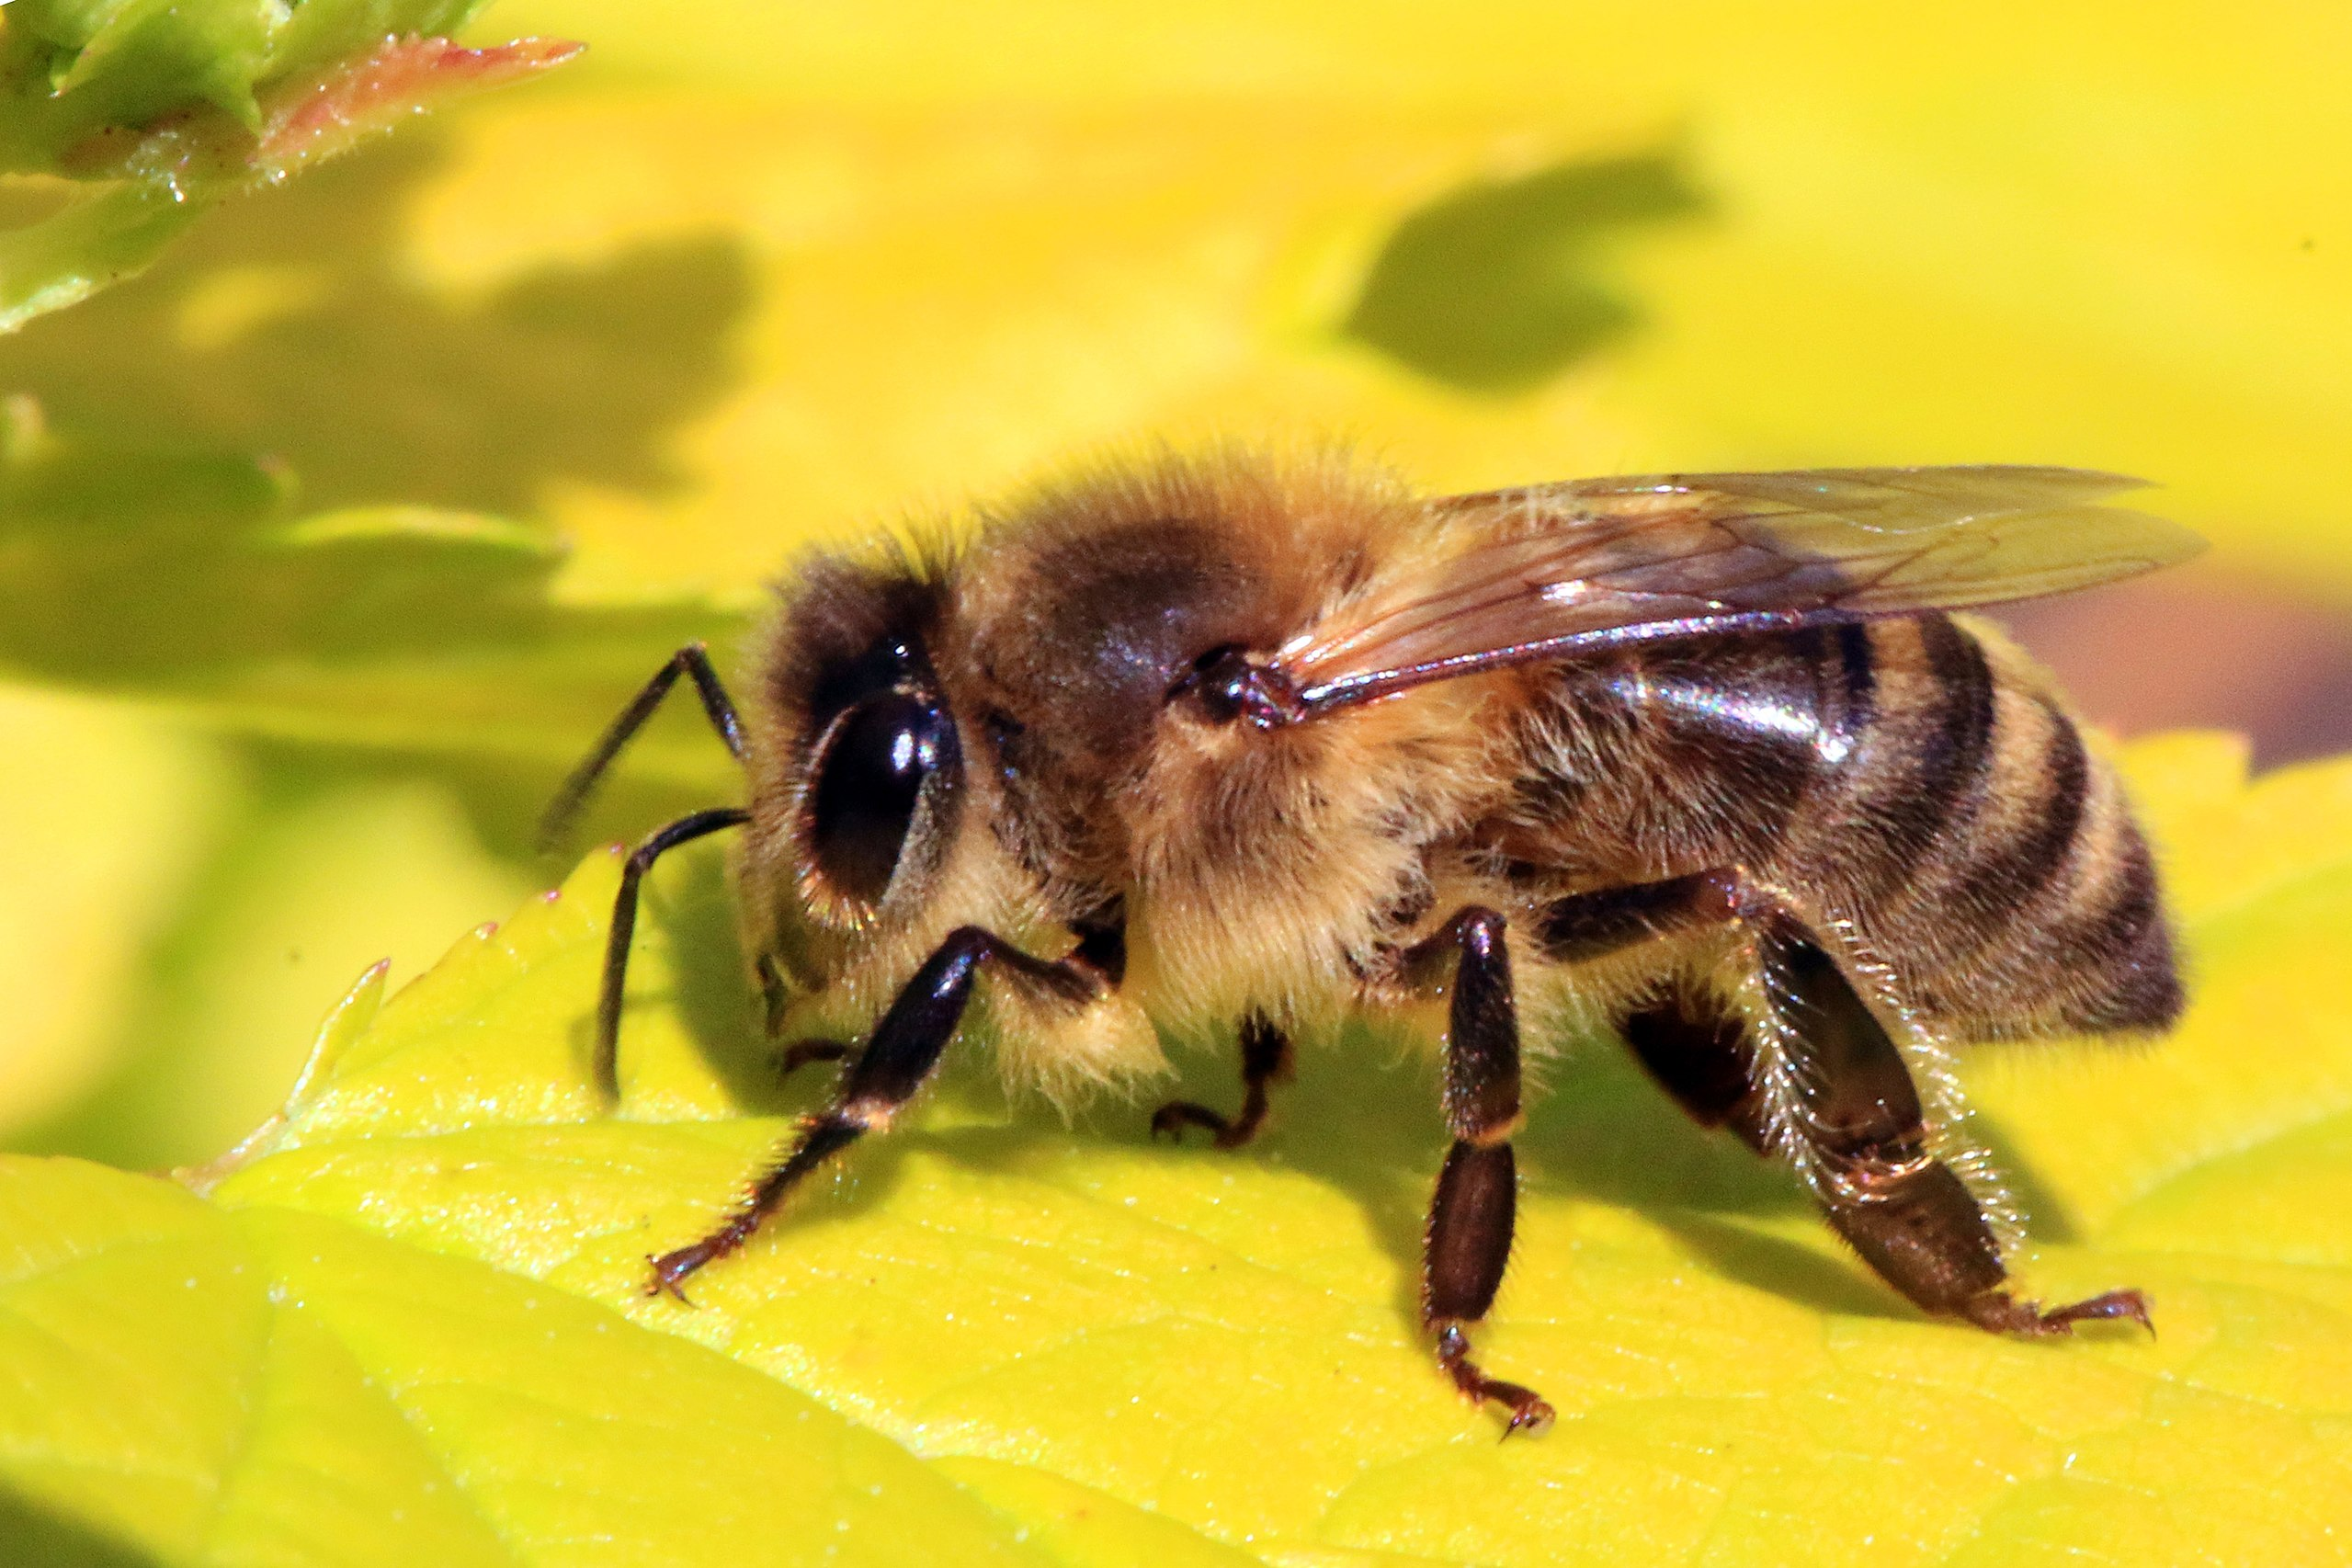
\includegraphics[scale=0.065]{./let_it_bee.jpg}
	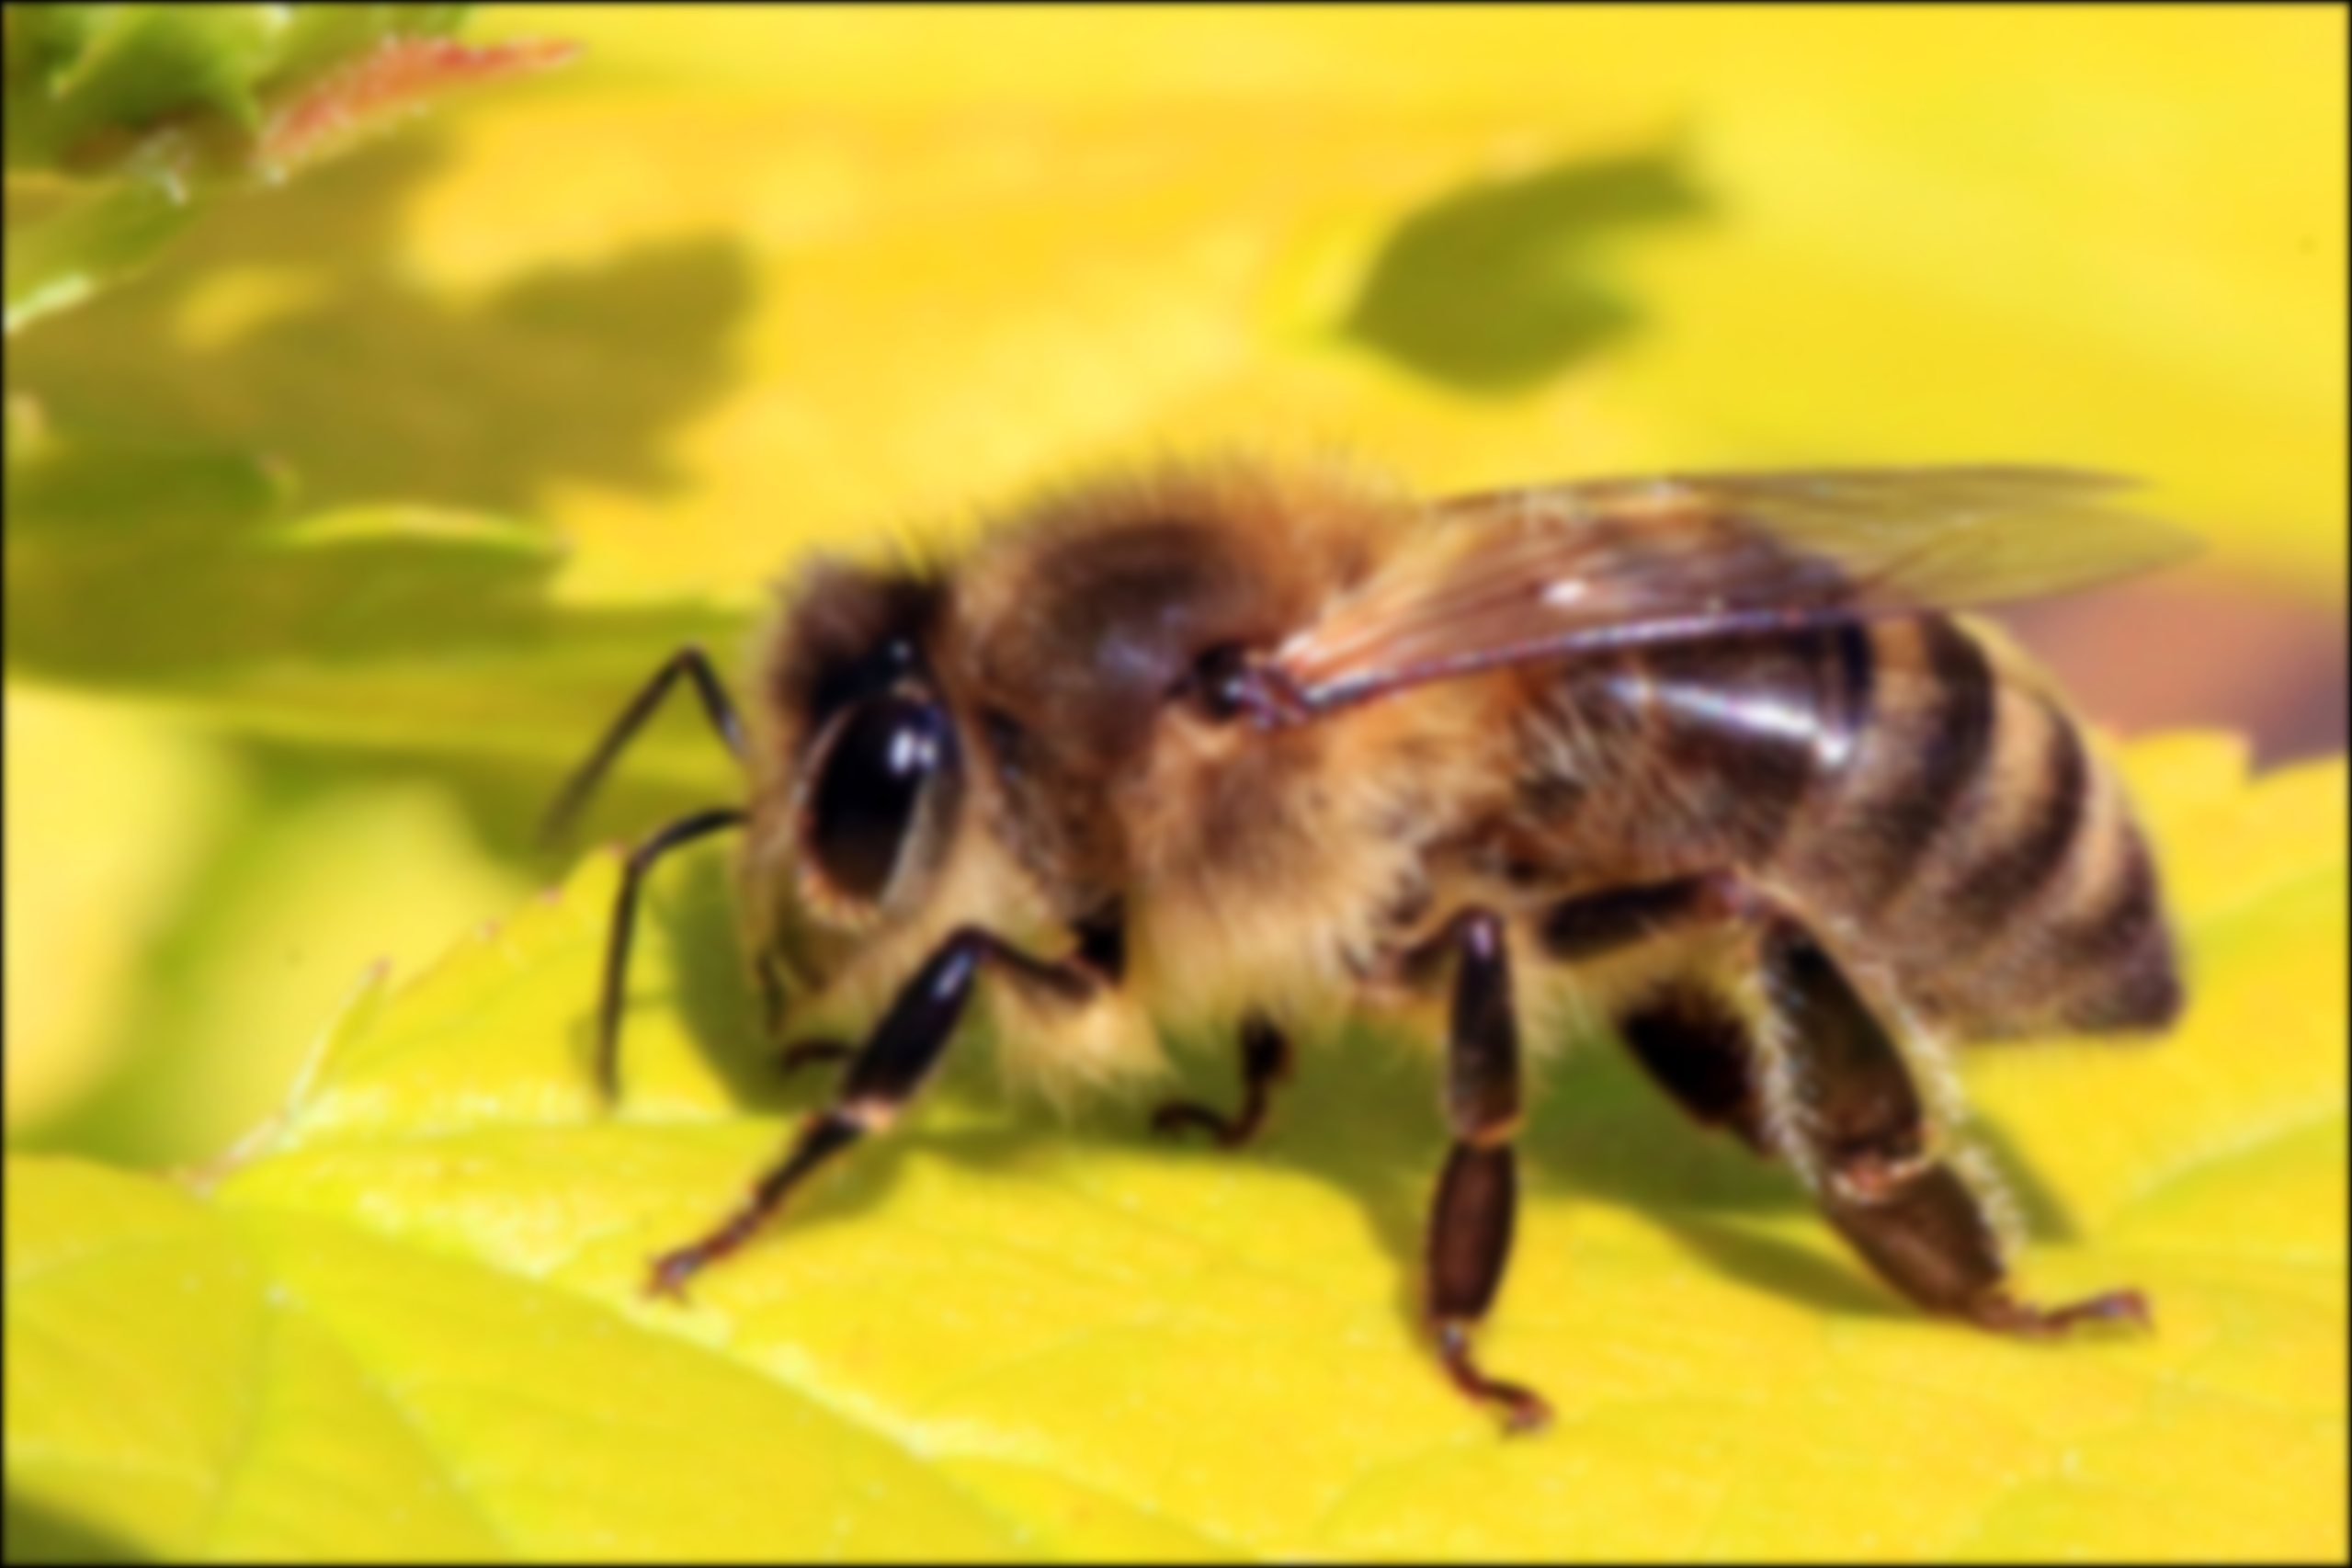
\includegraphics[scale=0.065]{./let_it_blur.png}
		\caption{A comparison displaying the effects of the blur. The left image is the original image, whereas the right image is the processed (blured) image.}
	\end{center}
\end{figure}

\begin{figure}[h!]
	\begin{center}
	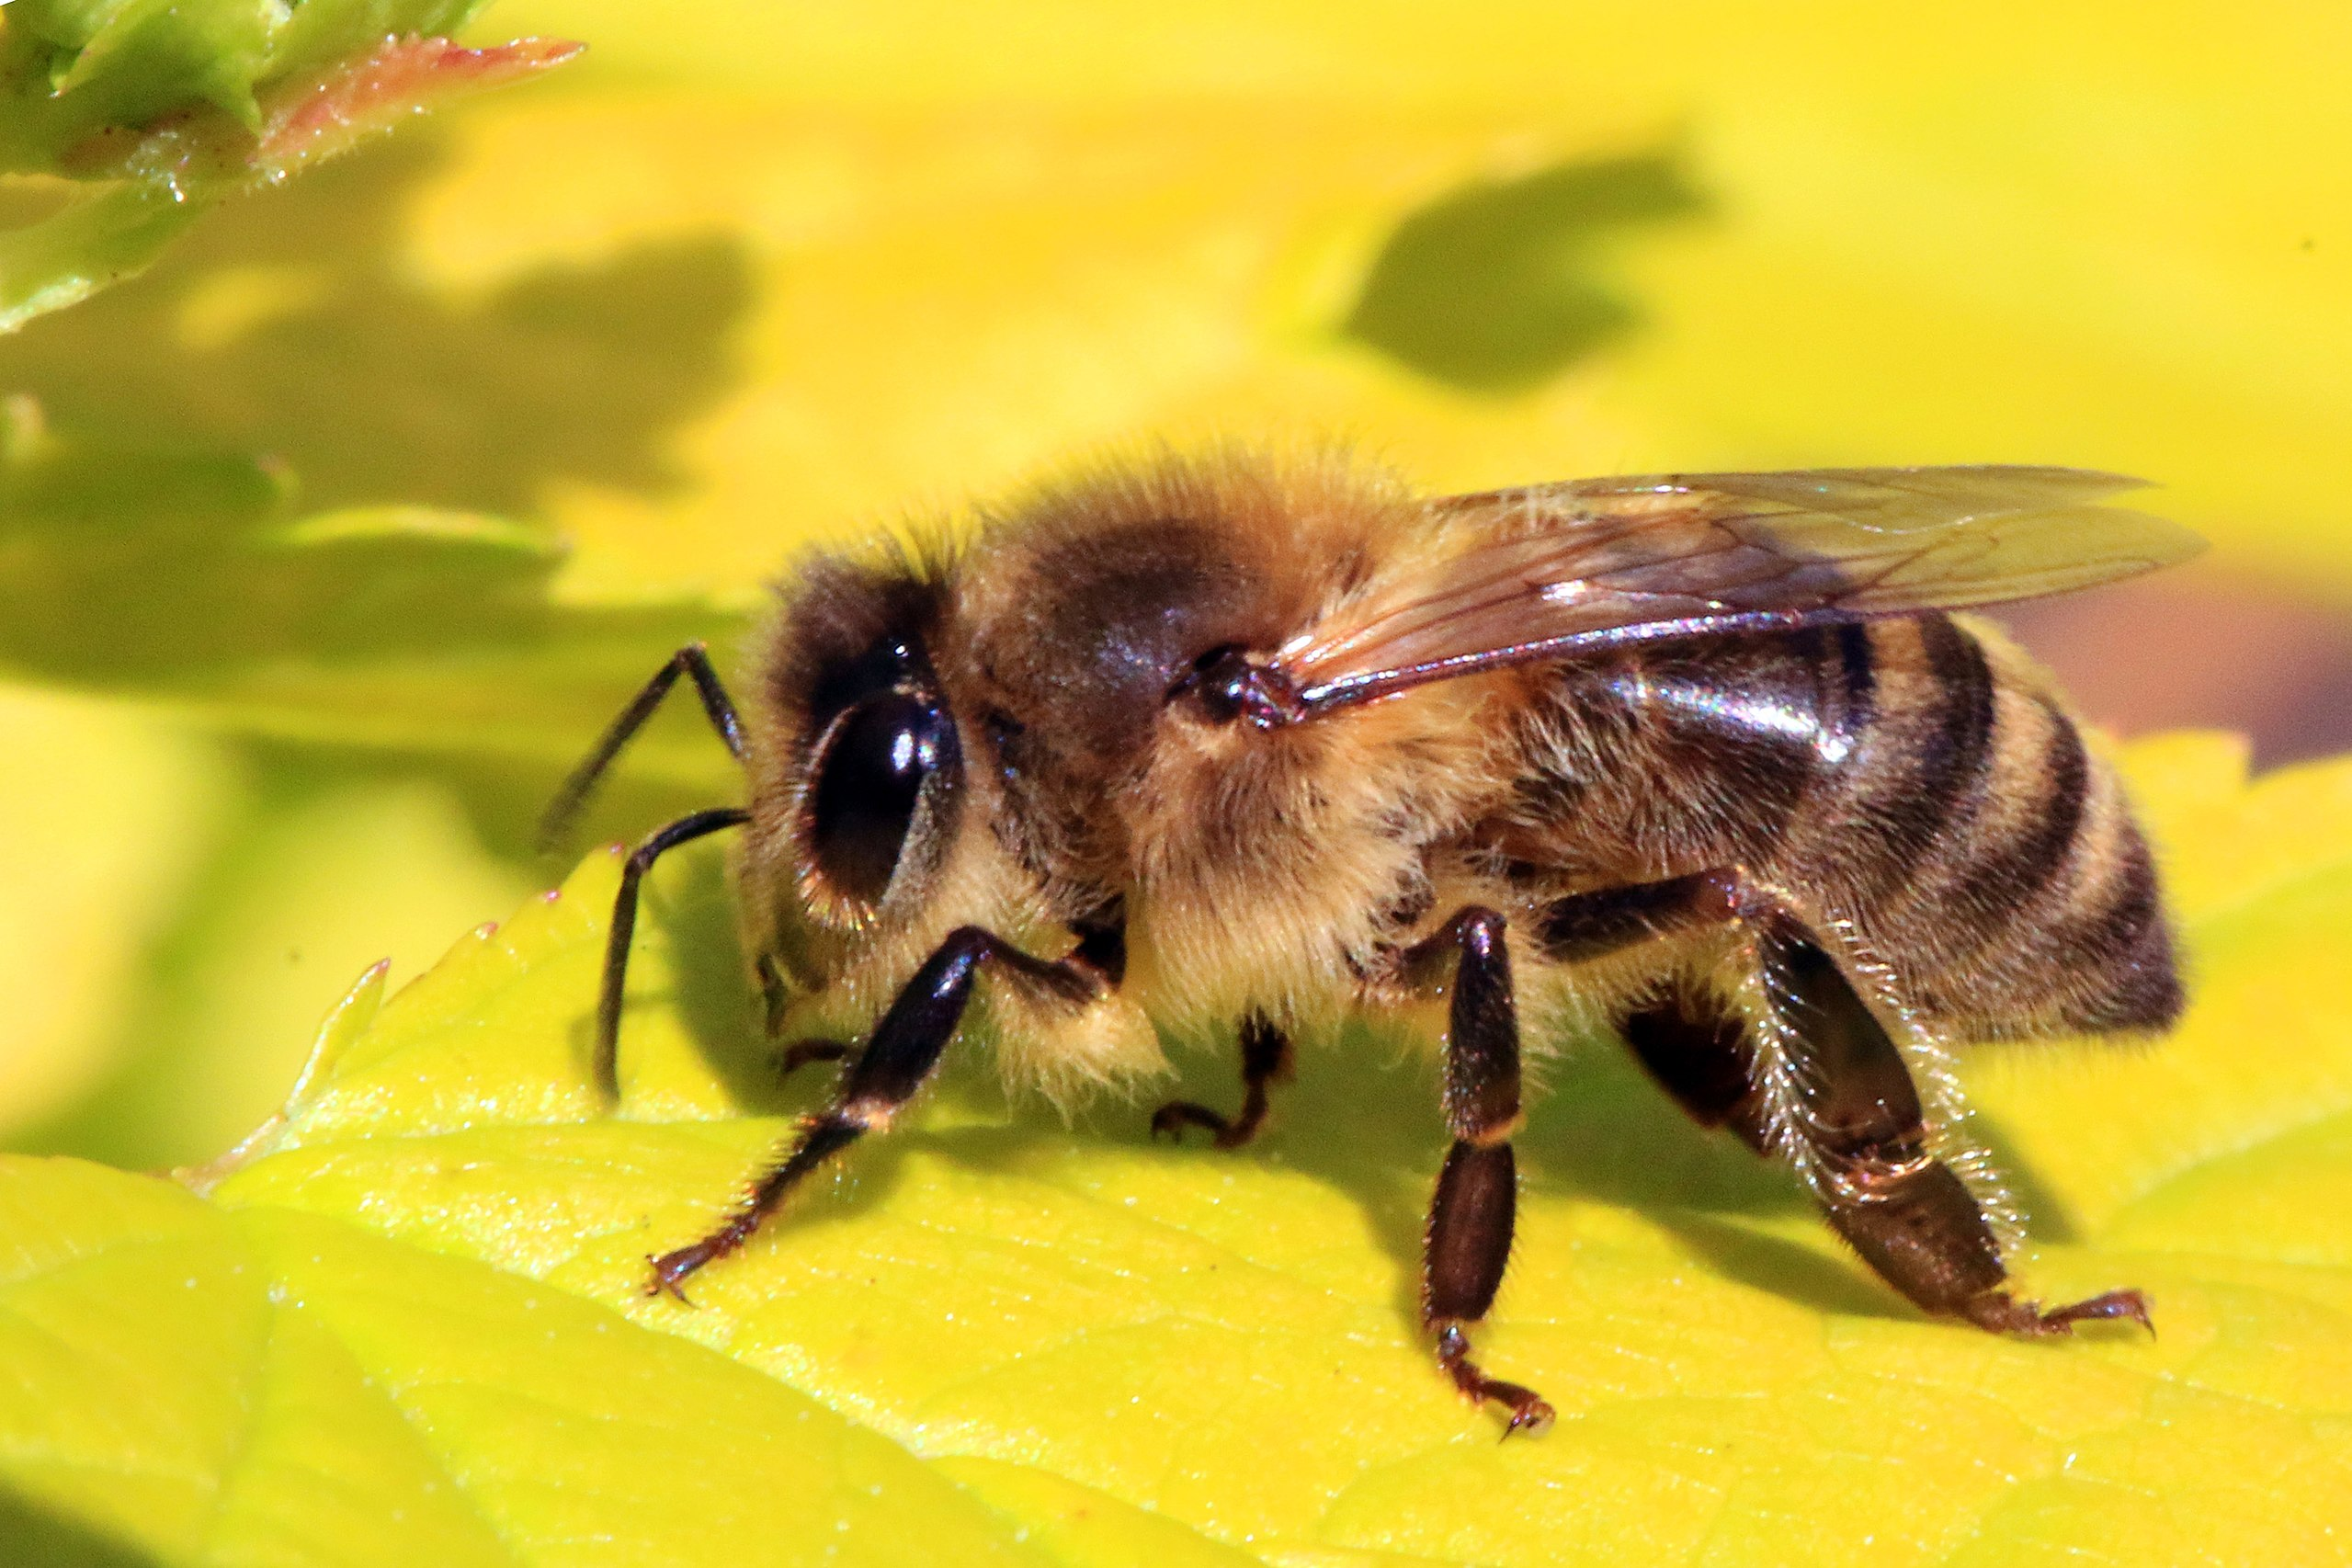
\includegraphics[scale=0.065]{./let_it_bee.jpg}
	\includegraphics[scale=0.065]{./let_it_sharpen.png}
		\caption{A comparison displaying the effects of the sharpening. The left image is the original image.}
	\end{center}
\end{figure}

\end{document}
